\subsection{Identificando Los Problemas, Estableciendo Acciones}

Ya con una manera de evaluar los estados observados de las aplicaciones definidas, lo siguiente a realizar era el establecer un proceso por el cual se pudieran identificar los problemas en la aplicación, y a partir de esto, establecer las acciones a realizar con el fin de modificar la arquitectura de la aplicación hacia el estado de referencia definido.

Como se estableció durante la sección \ref{sec:comparando}, el estado de la aplicación, en términos generales, es determinada por los estados de sus requerimientos de datos. Siendo así, se definió un proceso por el cual, a partir de las condiciones en las que se encuentren estos requerimientos, se determinen las acciones a realizar con el fin de adaptar la arquitectura.

% \begin{itemize}
%     \item \textbf{\textit{Addition}}: Busca crear nuevos componentes, a partir de servicios, con el fin de cumplir con las necesidades de datos.
%     \item \textbf{\textit{Restart}}: Esta acción está enfocada a reiniciar servicios que puedan haber fallado, con el fin de retornarlos a un estado funcional.
%     \item \textbf{\textit{Reconfigure}}: Busca el realizar cambios en componentes con el fin de cumplir con las necesidades establecidas.
% \end{itemize}

Partiendo de esto, se definió el proceso, descrito por la figura \ref{fig:BranProcess}, en dos partes. La primera, está encargada de la búsqueda e identificación de los problemas dentro de la aplicación; y la segunda, de manera interna, el determinar las acciones a seguir para adaptar la arquitectura. 

\begin{figure}[ht]
    \centering
    \caption{\\Proceso para la identificación de problemas de los requerimientos de datos}
    \label{fig:BranProcess}
    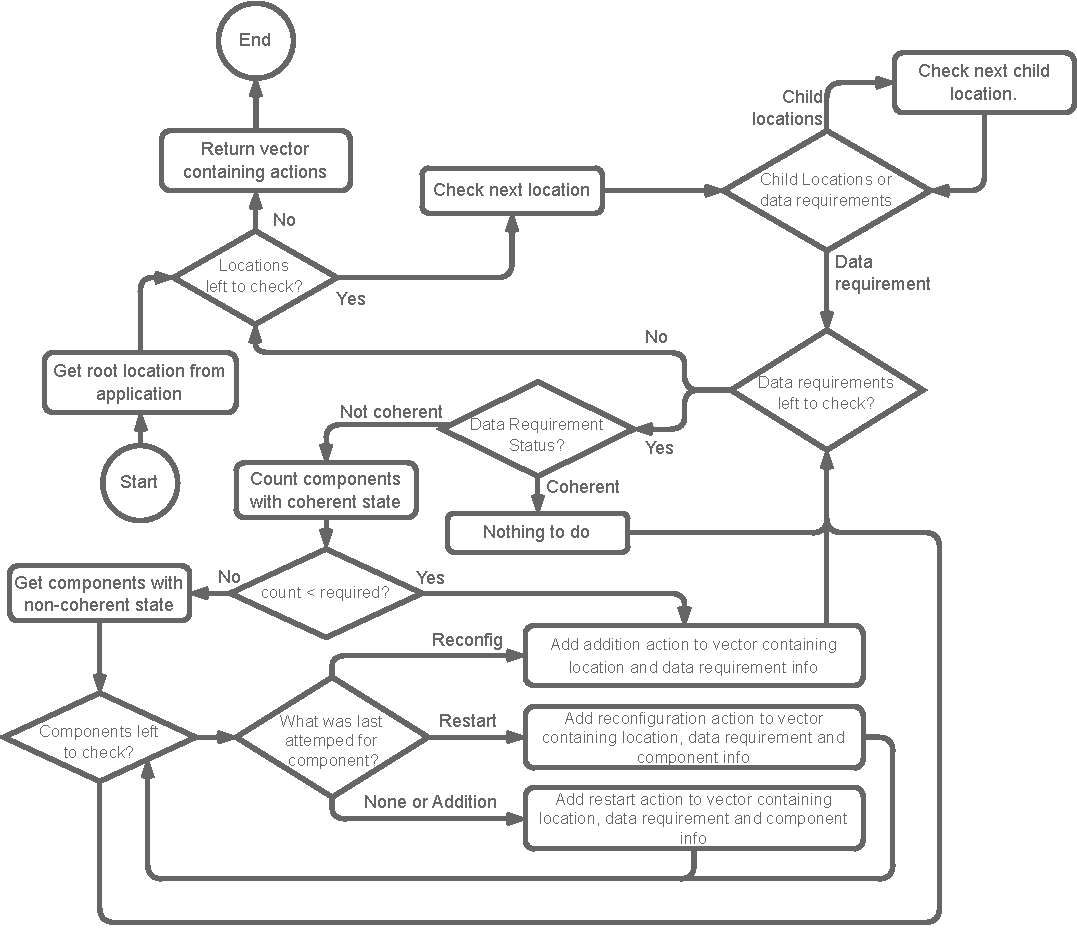
\includegraphics[width=0.9\linewidth]{images/BranProcessPlanner.pdf}
\end{figure}

La manera en la de que se identifican los problemas es similar a la vista en la figura \ref{fig:LookerProcessClock}. Se recorren las locaciones, buscando requerimientos de datos. Una vez en una de estas locaciones, se validan los requerimientos y se definen las acciones.

Ahora, las posibles acciones a tomar para la arquitectura de la aplicación, como se vió durante la sección \ref{sec:MecAdap}, dependen de los objetivos y los requerimientos del sistema. Siendo así, se tomaron 3 tipos de acciones por las cuales se puede modificar el estado del sistema: \textit{Addition}, \textit{Restart} y \textit{Reconfigure}.

Todos los requerimientos en un estado diferente a \textit{Coherent}, son evaluados con el fin de establecer la acción a realizar. Lo primero, es revisar la cantidad de componentes registrados en el requerimiento; si se tiene menos de los requeridos, se realizará un acción tipo \textit{Addition} con el fin de cumplir con el numero de fuentes de datos esperada.

En el caso de tener la cantidad requerida de dispositivos, pero estado aún en estado \textit{Fault}; la siguiente opción es reiniciar el servicio. Esto busca poner nuevamente en un estado válido el componente, en caso de que haya quedado en un estado inválido; o poner nuevamente en ejecución el servicio en el escenario de que este haya muerto.

Si el reiniciar no tiene efecto en el estado del componente, la siguiente opción es reconfigurar el componente. Esto busca la modificación de algún aspecto, sea la actualización una variable de ambiente o parámetro, con el fin de retornarlo a un estado válido. 
 
Finalmente, si todo falla y no es posible recuperar el dispositivo; la última opción es iniciar un nuevo servicio el cual pueda suplir las condiciones de su predecesor. De esta manera, aún es posible retornar la aplicación hacia un estado válido, independiente de los componentes en un estado irrecuperable.

La implementación de este proceso, se realizó en el agregador \textit{Bran}. Esto debido a que, al tener el estado de las aplicaciones, cortesía de lo observado por \textit{Looker}; deja a este servicio como el punto medio de la aplicación, encargado de definir las acciones a realizar.